\section{Seblstreparatur in Biologie und Technik}

\subsection{Selbstreparatur in der Natur}

\textit{Wo findet man geeignete Lösungen von Selbstreparatur in der Natur?}

\begin{center}
    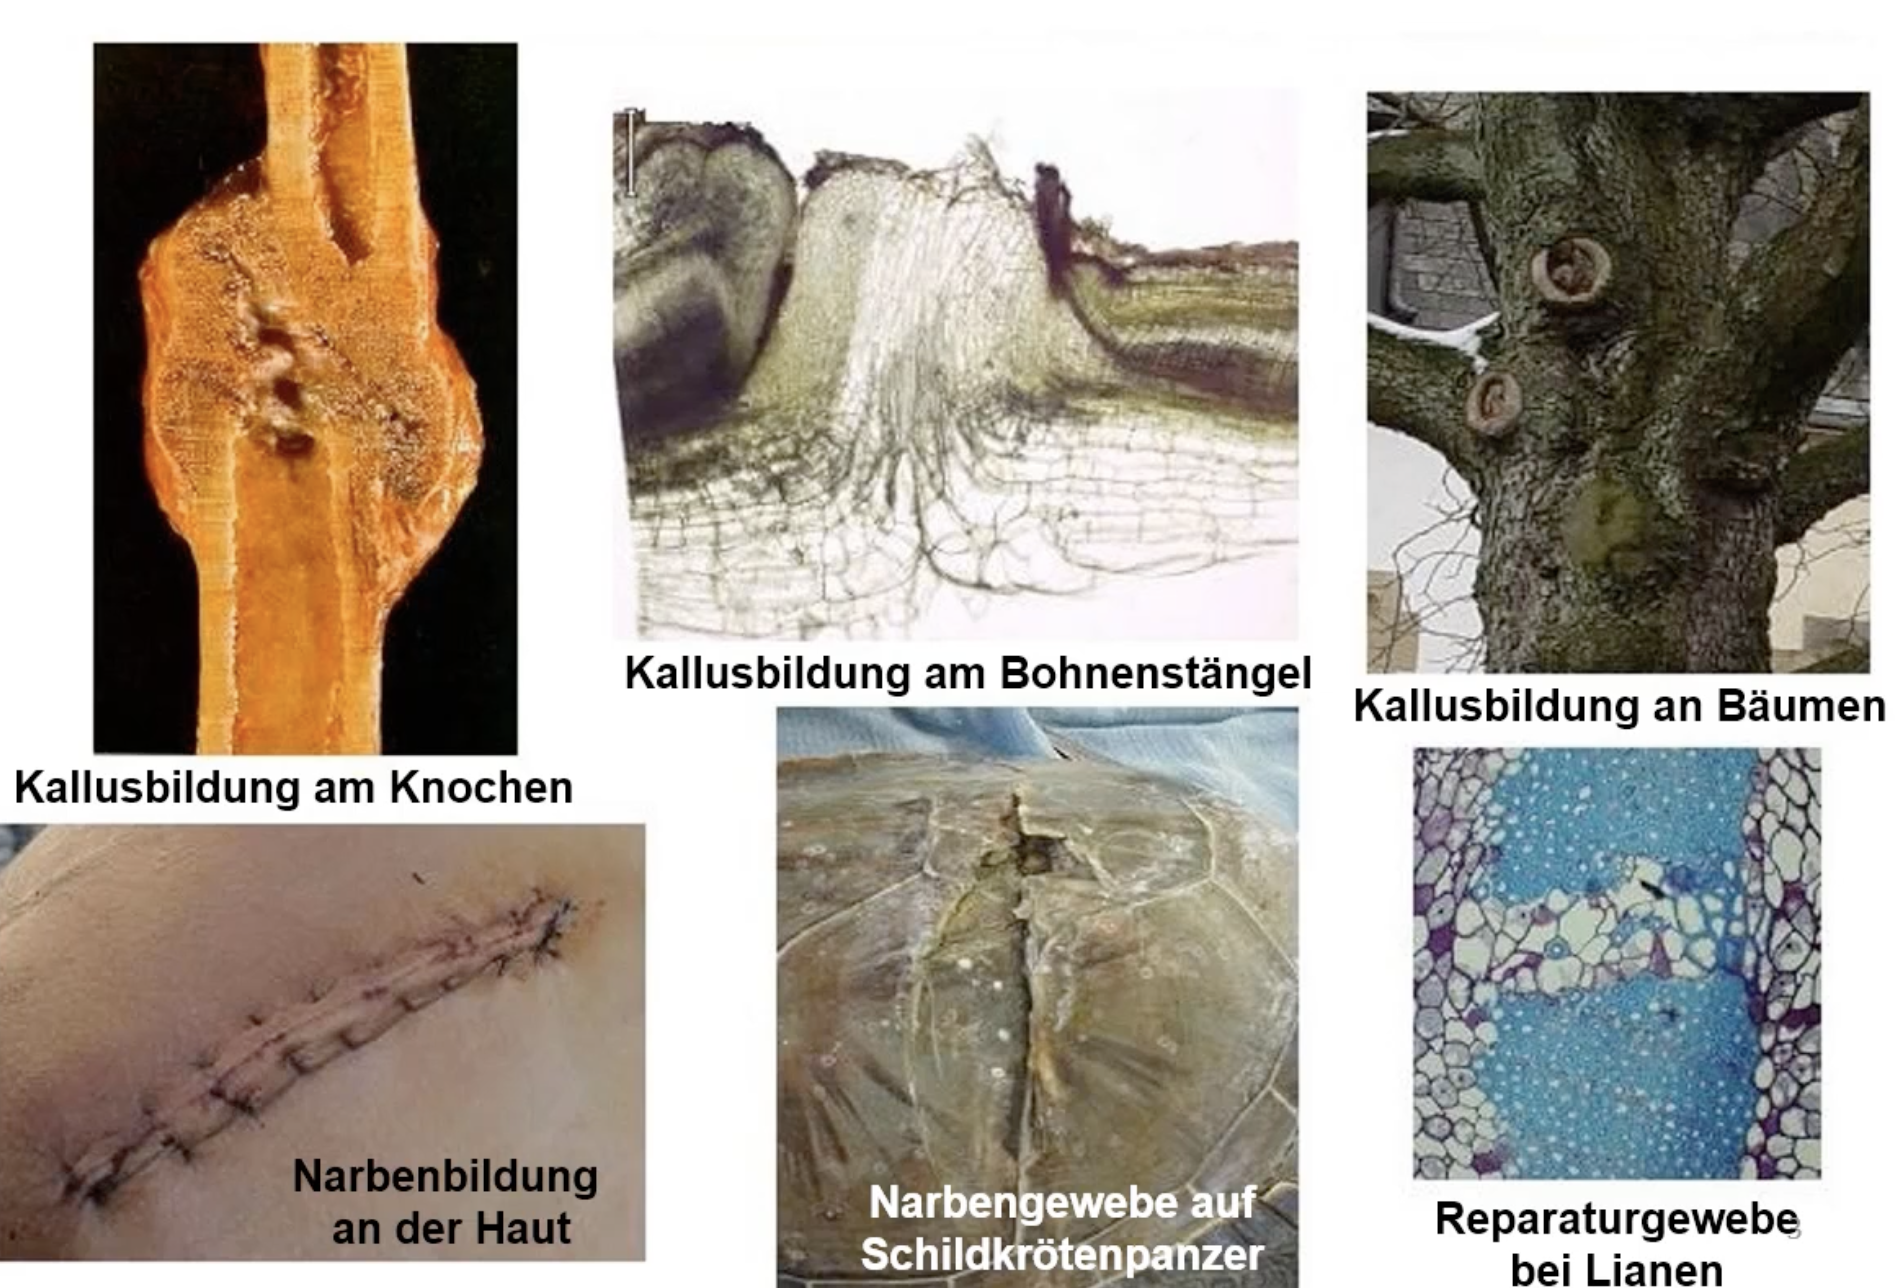
\includegraphics[width=12cm]{lec5/figures/selbstheilung-natur.png}
\end{center}

\begin{itemize}
    \item Kallusbildung am Knochen: Durch Zellwachstum werden die gebrochenen Teilstücke wieder zusammengeführt und sind danach stärker als zuvor (ein Knochen bricht niemals an derselben Stelle zweimal). \item Dadurch wird der Knochen allerdings schwerer.
\end{itemize}

\subsection{Selbstreparatur in der Technik}

\textit{Welche bestehenden Lösungen gibt es bereits in der Technik?}

\begin{center}
    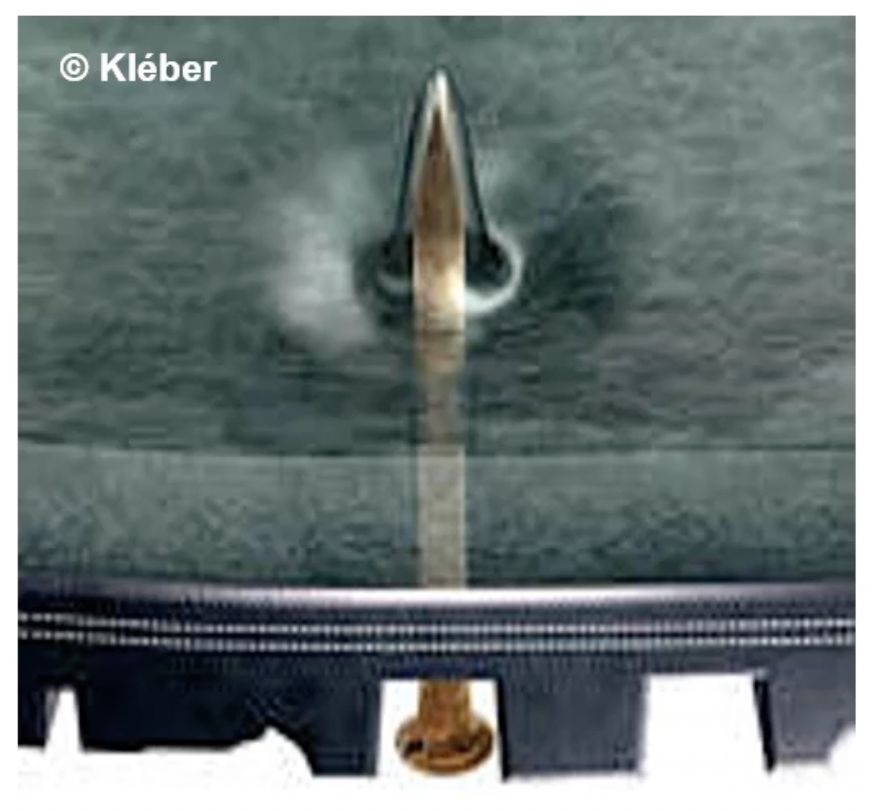
\includegraphics[width=5cm]{lec5/figures/selbstheilung-technik-1.png}
    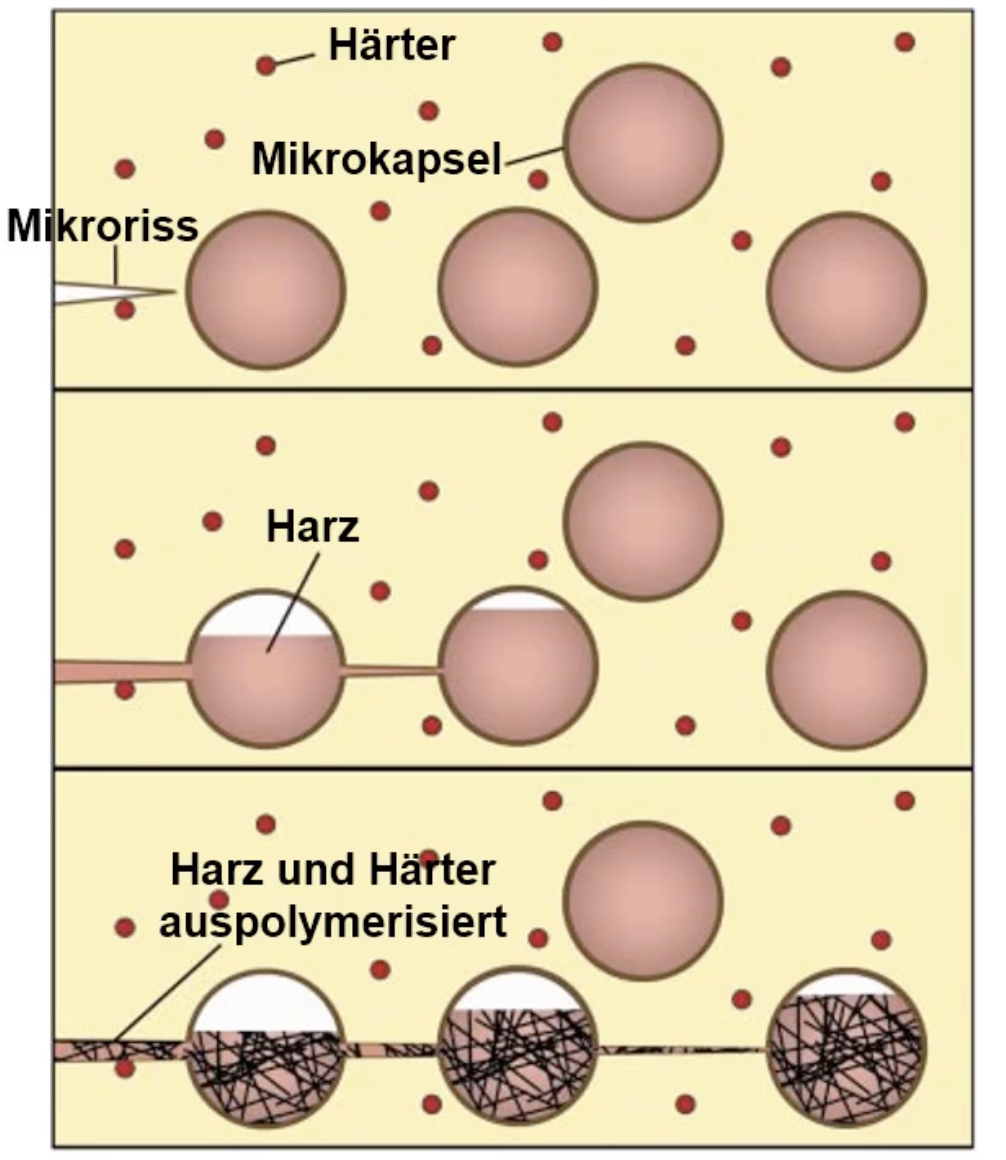
\includegraphics[width=5cm]{lec5/figures/selbstheilung-technik-3.png}
    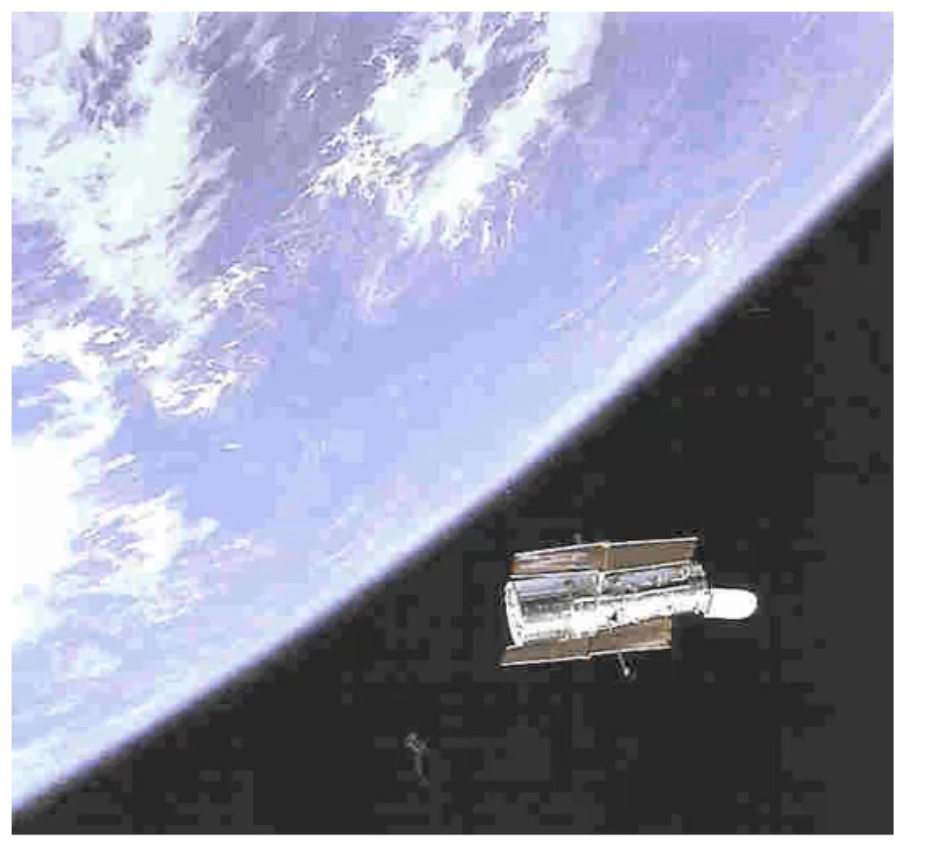
\includegraphics[width=5cm]{lec5/figures/selbstheilung-technik-4.png}
\end{center}

\begin{itemize}
    \item Reifendichtungsmittel (kein Bild): Kurzfristiger Reparatureffekt durch zähflüssige Emulsion mit synthetischen Fasern innerhabl des Reifens.
    \item \textbf{Selbstreparierender Autoreifen} (links): Bei punktartiger Verletzung der Struktur (bis 4,7 mm) zieht sich das Gewebe des Polymers aufgrund der Molekularstruktur zusammen und dichtet das Loch ab. 
    \item \textbf{Sebstreparierende spröde Polymere} (mitte): Struktur ist von Mikrokapseln mit Harz sowie kleinen Härterkügelchen durchsetzt. Werden beide angestochen und treffen aufeinander (durch Kappilareffekte), kommt es durch die 2-Komopenten-Wirkung zur Aushärtung.
    \item Organischer Beton (kein Bild): Beton, in welchen gefriergetrocknete Bakterien eingebracht werden, welche bei Eindringen von Fremdkörpern (z. B. Wasser) wachsen und Stoffe absondern, die den Beton "kitten".
    \item \textbf{Selbstreparierende Materialien für die Raumfahrt} (rechts): Verhinderung von Luftaustritt. Einziges bionisches Beispiel in dieser Auflistung, entwickelt nach Vorbild der menschlichen Blutgerinnung. Im Abschnitt ``Selbstreparatur in der Bionik'' beschrieben.
\end{itemize}

\subsubsection{Zweikomponentensysteme}

\textbf{Analyse der selbstreparierenden spröden Polymere}\\

\begin{center}
    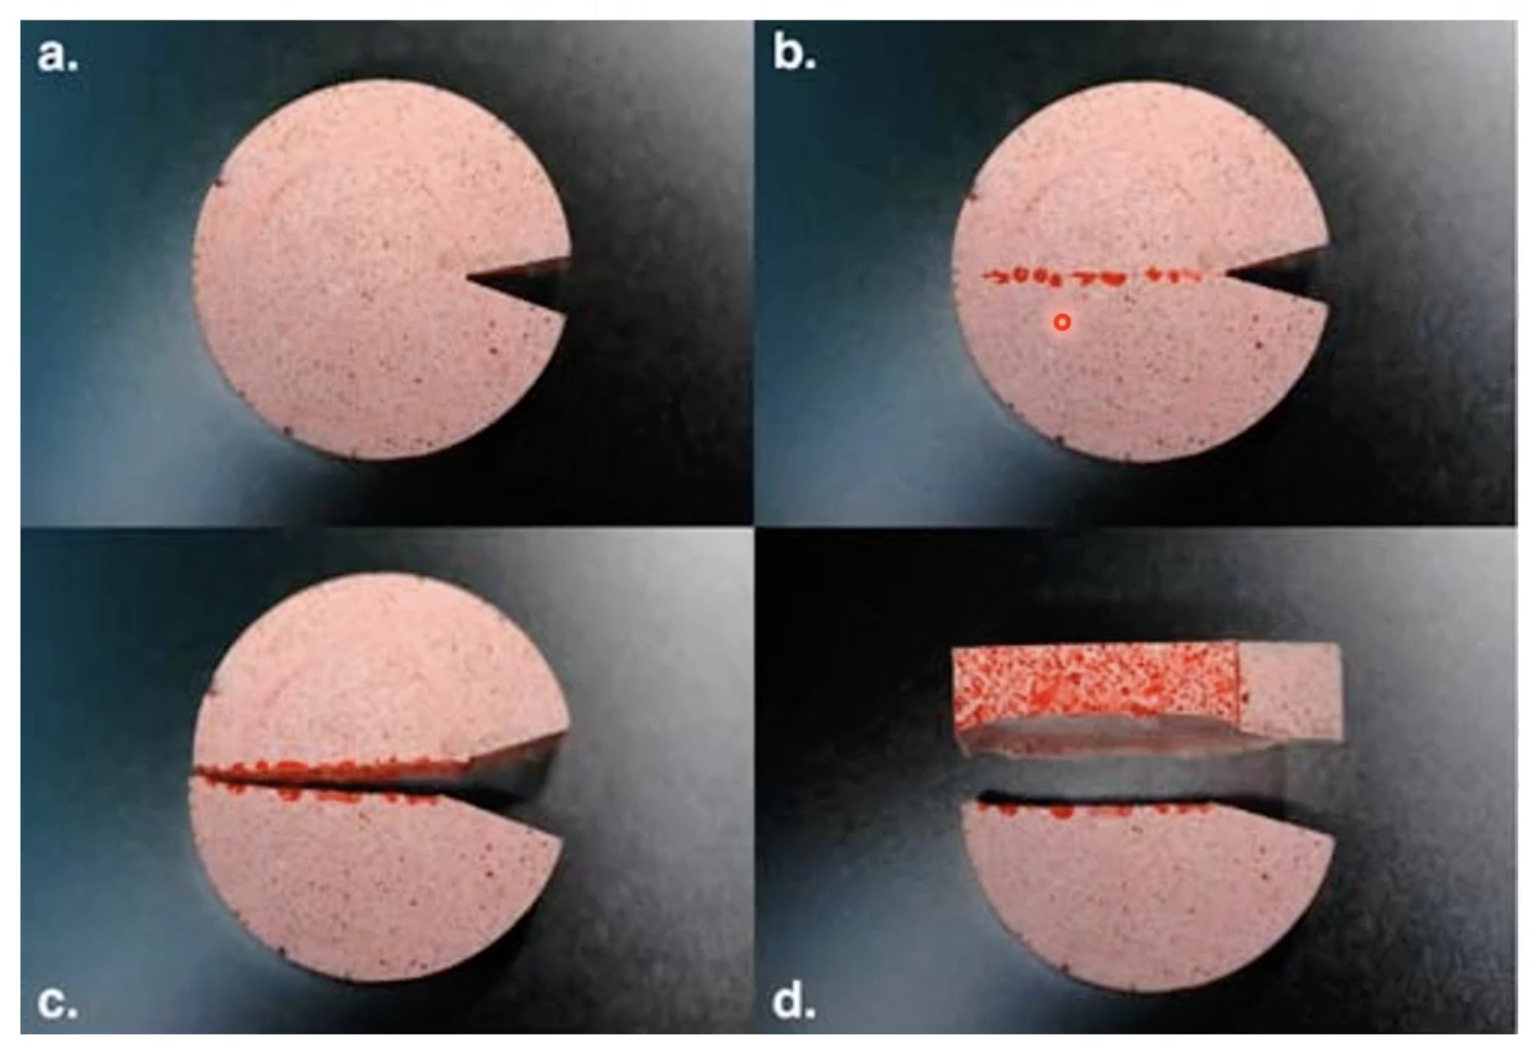
\includegraphics[width=7cm]{lec5/figures/selbstheilung-technik-2.png}
    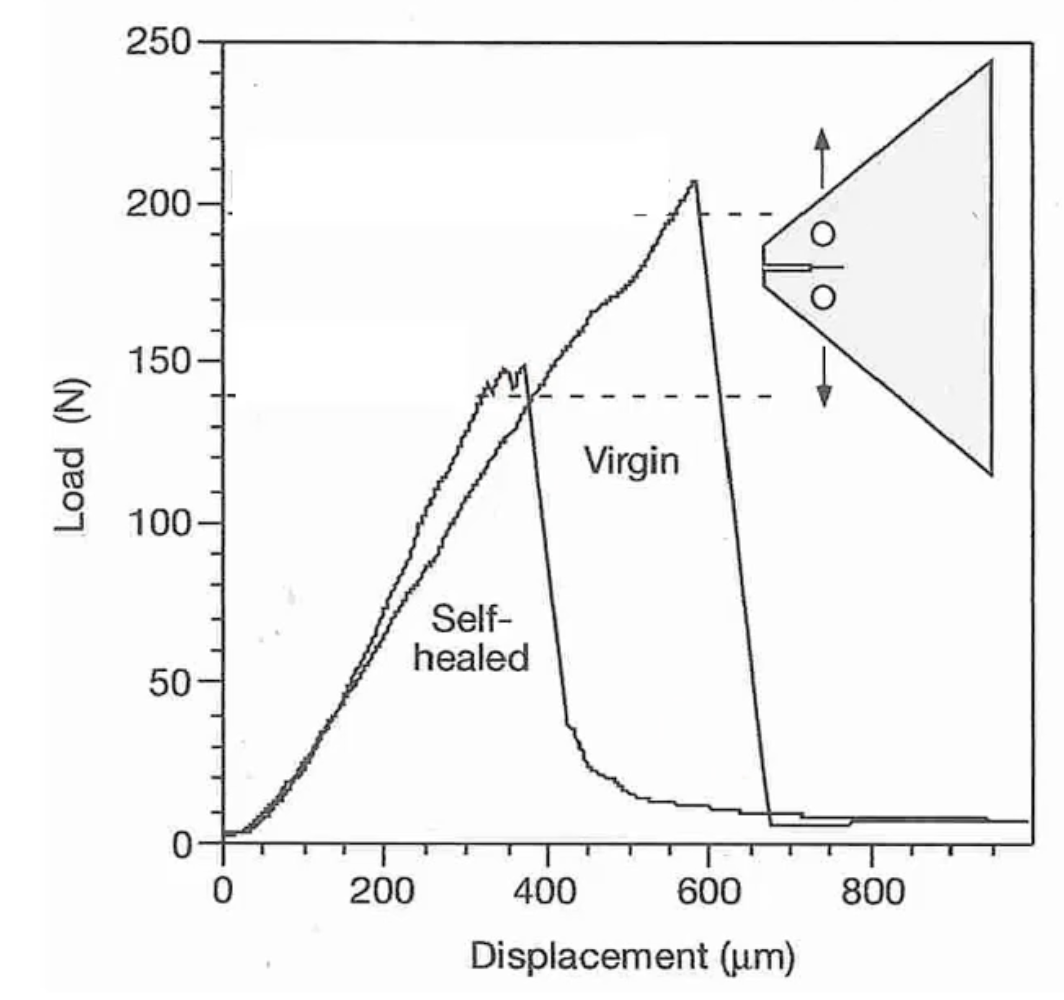
\includegraphics[width=6cm]{lec5/figures/zugversuch.png}
\end{center}

\begin{itemize}
    \item Optische Analyse mit REM, anhand derer der Kapillareffekt sichtbar sowie die Bruchstelle analysiert wird.
    \item Quantitfizierung anhand von Zugversuchen (siehe Kraft-Weg-Diagramm), 60\% der Bruchlast des selbstgeheilten Materials im Vergleich zum unbeschädigten Probenkörper.
\end{itemize}

\subsubsection{Quellende Hydrogele}

Neben den Zweikomponentensysteme mit zwei synthetischen Komponenten kommen auch Hydrogele (\textbf{SAP = superabsorbierende Polymere}) in den selbstreparierenden und -abdichtenden Materialien der Technik zum Einsatz, welche als zweite Komponente die Umgebungsfeuchte bzw. das Medium, gegen welches sie abdichten nutzen. Diese können enorm viel Feuchtigkeit aufnehmen und dadurch bis zur 1000-fachen Masse isotrop quellen. Sie kommen in Alltagsverbrauchsgütern z. B. bei Windeln, im technischen Einsatzgebiet bei Dichtungen zum Einsatz.\\

\begin{center}
    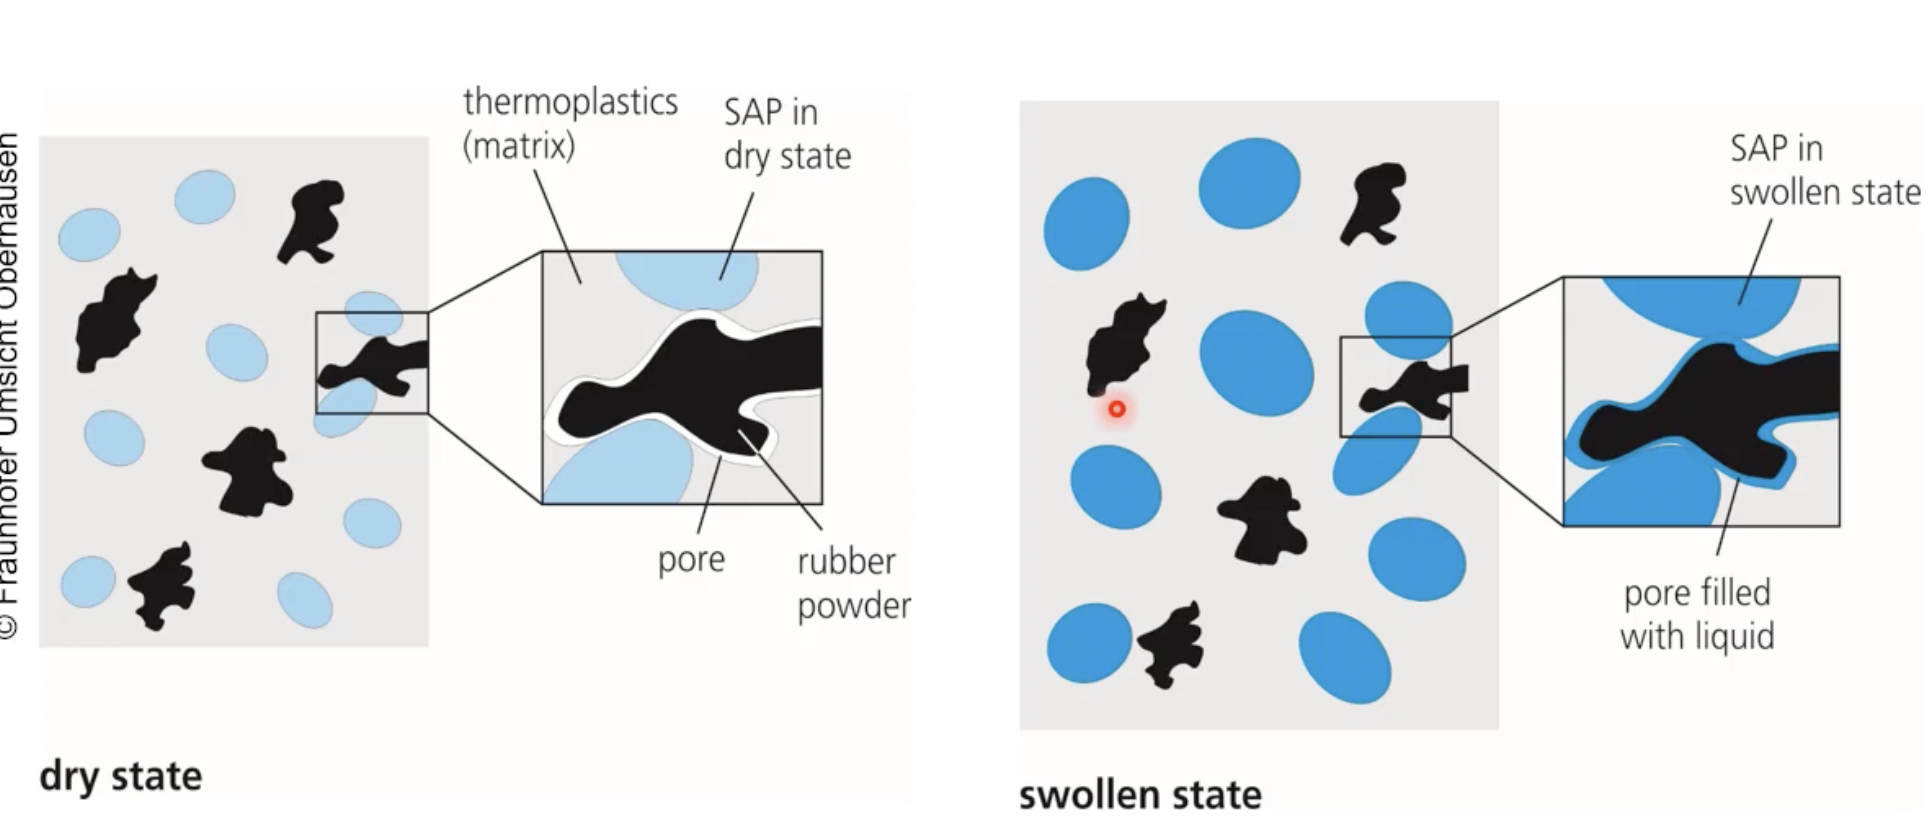
\includegraphics[width=14cm]{lec5/figures/TPE.png}
\end{center}

Diesen Effekt machen sich die \textbf{thermoplasitschen Elastomerkomposite} zu Nutzen, welche aus Gummipuder, SAP und Thermoplaste bestehen. Gummipuder und SAP sind dabei in eine Thermoplast-Matrix eingelassen (Bild). Sie haben ähnliche Eigenschaften wie Gummi, lassen sich ähnlich produzieren wie Thermoplaste (flexible Formgebung), quellen isotrop wie SAP und lassen sich hervorragend recyclen. Ein Anwendungsfall hierfür ist der Dichtschlauch Tangit.\\

Ein Nachteil quellfähiger Dichtungen ist, dass die Quellung nicht auf den Rissbereich beschränkt ist, wodurch die Formstabilität der Dichtung leidet. Dem wird vorgebeugt, indem die Dichtung durch einen speziellen Einbau von formstabilem Material umschlossen wird.

\subsection{Selbstreparatur in der Bionik}

\subsubsection{Abdichtung nach Vorbild der menschlichen Blutgerinnung}

Selbstreparierende Materialien in der Raumfahrt nach Vorbild der Blutgerinnung im menschlichen Körper.

\textbf{Blutgerinnung im menschlichen Körper.} (Nicht im Detail für die Klausur notw.)

\begin{enumerate}
    \item Fremdkörper oder Riss verletzt Integrität des Blutgefäßes.
    \item Blut tritt aus Blutbahn aus und kommt mit Gewebe in Kontakt.
    \item Sensorik in Haut registriert Blut und startet durch Gewebe- und Plasmafaktoren die Blutgerinnungskaskade.
    \item Enzyme werden kaskadenartig (und damit selbstverstärkend) produziert, welche wiederum neue Enzyme produzieren, bis Fibrin hervorgerufen wurde.
    \item Fibrinfasern vernetzen und bilden mit Thrombozyten und roten Blutkörperchen einen Thrombus, der die Wunde verschließt.
\end{enumerate}

\begin{center}
    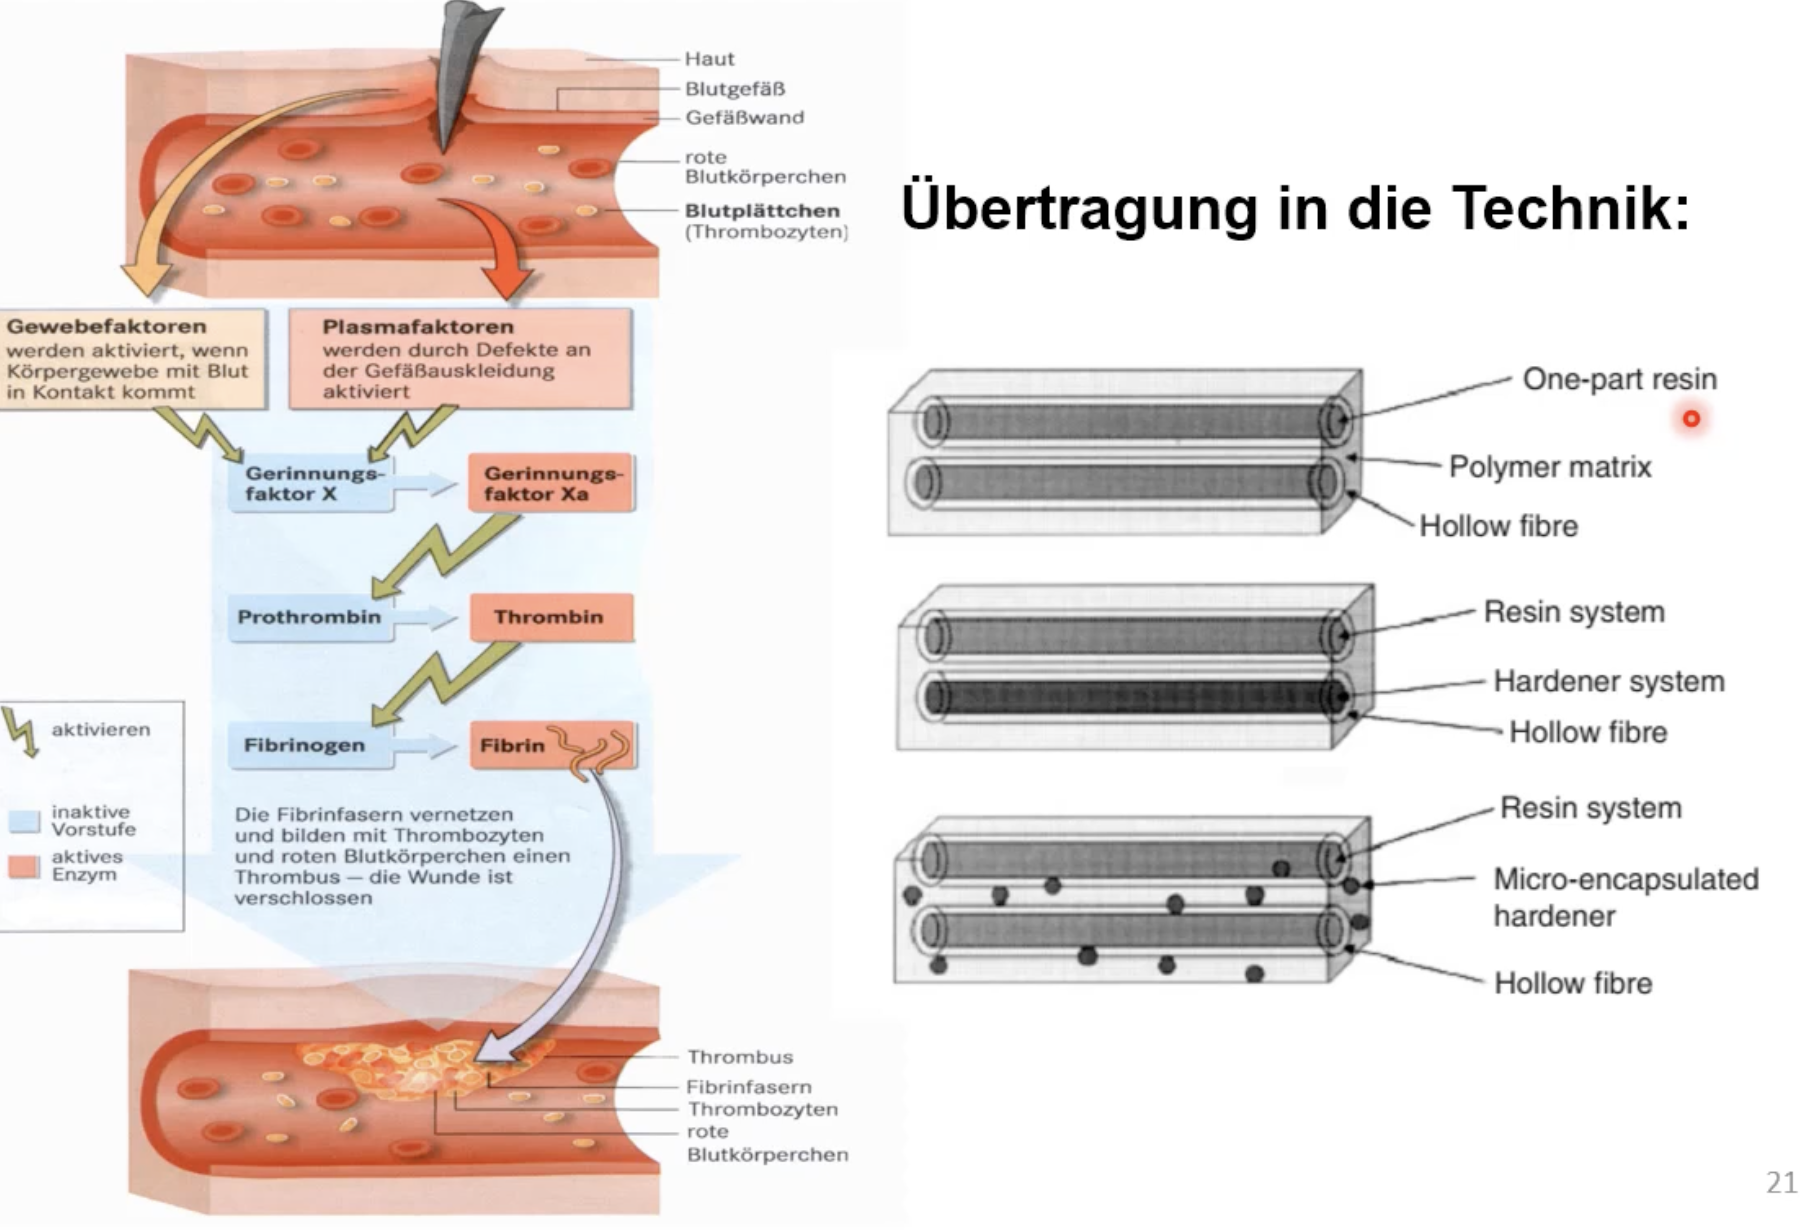
\includegraphics[width=14cm]{lec5/figures/blutgerinnung.png}
\end{center}

Ein Nachteil des Blutgerinnungsprozess ist es, dass nach Wundheilung die wieder abgelösten Fibrinfasern in \textbf{Engstellen des Blutkreislaufes} stekenbleiben können (z.B. durch Fett verkalkte Gefäße oder schmale Herzkranzgefäße). Durch Verstopfung kann kein Sauerstoff mehr zu den hintergeschalten Zellen geführt werden, was im Herzen zum Herzinfarkt, im Gehirn zum Schlaganfall und in den Gliedmaßen zur Thrombose führen kann.\\

Die Vielzahl an Kaskaden hat folgende Notwendigkeiten:

\begin{itemize}
    \item Verstärkung der Reaktion, da Enzyme schnell reaktiviert werden können. Ein Enzym aktiviert mehrere Zielproteine.
    \item Vermeidung von Fehlreaktionen.
\end{itemize}

Für die \textbf{bionische Abbildung des Blutgerinnungsprozesses im Rahmen der Raumfahrt} zur Vermeidung von Lufteintritt wurde ein Zweikomponentensystem genutzt, bestehend aus Hohlfasern mit Resin, Härter-Mikrokapseln, welche in den Zwischenräumen eingelagert sind, und Glasfasern (siehe Bild, rechts unten) \dangersign.
\\\\
\textbf{Zusammenfassung}:

\begin{itemize}
    \item Blutgerinnung als Vorbild für selbstheilenden Materialien in der Raumfahrt \dangersign
    \item Blutgerinnung funktioniert über Signalkaskade (Verstärkung + Vermeidung von Fehlreaktionen)
    \item Übertragung auf Technik durch 2-Komponenten Kunstharzsystem
    \item Kunstharz wird zusammen mit UV-Farbstoff in Hohlfaser gegeben
    \item Anordnung der Hohlfasern in Verbundmatrix mit Glasfasern
    \item Hohlfasern sind in 90° Winkel zu Glasfasern ausgerichtet
    \item Gezielte Schadensanalyse durch Biegetest
    \item Unbeschadetes selbstheilendes Material hat geringere Biegefestigkeit als Material ohne Selbstheilungsfunktion
    \item Biegefestigkeit ist nach Schadensereignis vollständig wieder hergestellt
    \item UV-Farbstoff ermöglicht visuelle Überprüfung des Materials auf Schäden
    \item Aushärten erfordert hohe Temperaturen und viel Zeit
\end{itemize}

\subsubsection{Abdichtung nach Vorbild des biochemischen Wundverschlusses bei Pflanzen}

Als Motivation für diese bionische Forschung dienen Polymere in Anwendungen mit hoher mechanischer Belastung, bei denen ein Versagen von Konstruktionen auftritt, bevor die eigentliche Beanspruchungsgrenze erreicht ist. Die \textbf{intrisisch aktivierte} Selbstreparatur nach Vorbild des biochemischen Wundverschlusses bei Pflanzen dient dazu, plötzlichem Versagen durch unkontrolliert wachsende Mikrorisse vorzubeugen \dangersign.\\

\textbf{Biologische Vorbilder} für dieses Vorgehen sind pflanzliche Sekrete und die für ihren Transport und ihre Speicherung zuständigen Gewebe und Zellen. 

\begin{itemize}
    \item \textbf{Sekrete} sind Milchsäfte (Ficus benjamina, Löwenzahn, Lotusblume, Schlafmohn, Würgefeige) und Harze (Kautschuk, Guttapercha, Gummi arabicum, Schellack als Ausscheidungen von Blattläusen, Balsam, Kiefern).
    \item \textbf{Transport- und Speichersysteme} sind Mikroröhren (Milchröhren, Harzgänge) oder spährische Harzbehälter/Mikrokapseln.
\end{itemize}
Baumharze härten aus, wenn die darin vorhanden \textbf{Turpentin-Öle} verdunsten. Durch die erneute Zugabe von Turpentin bzw. Terpentin kann der Harz wieder verflüssigt werden (Lösungsmittel).\\

\begin{center}
    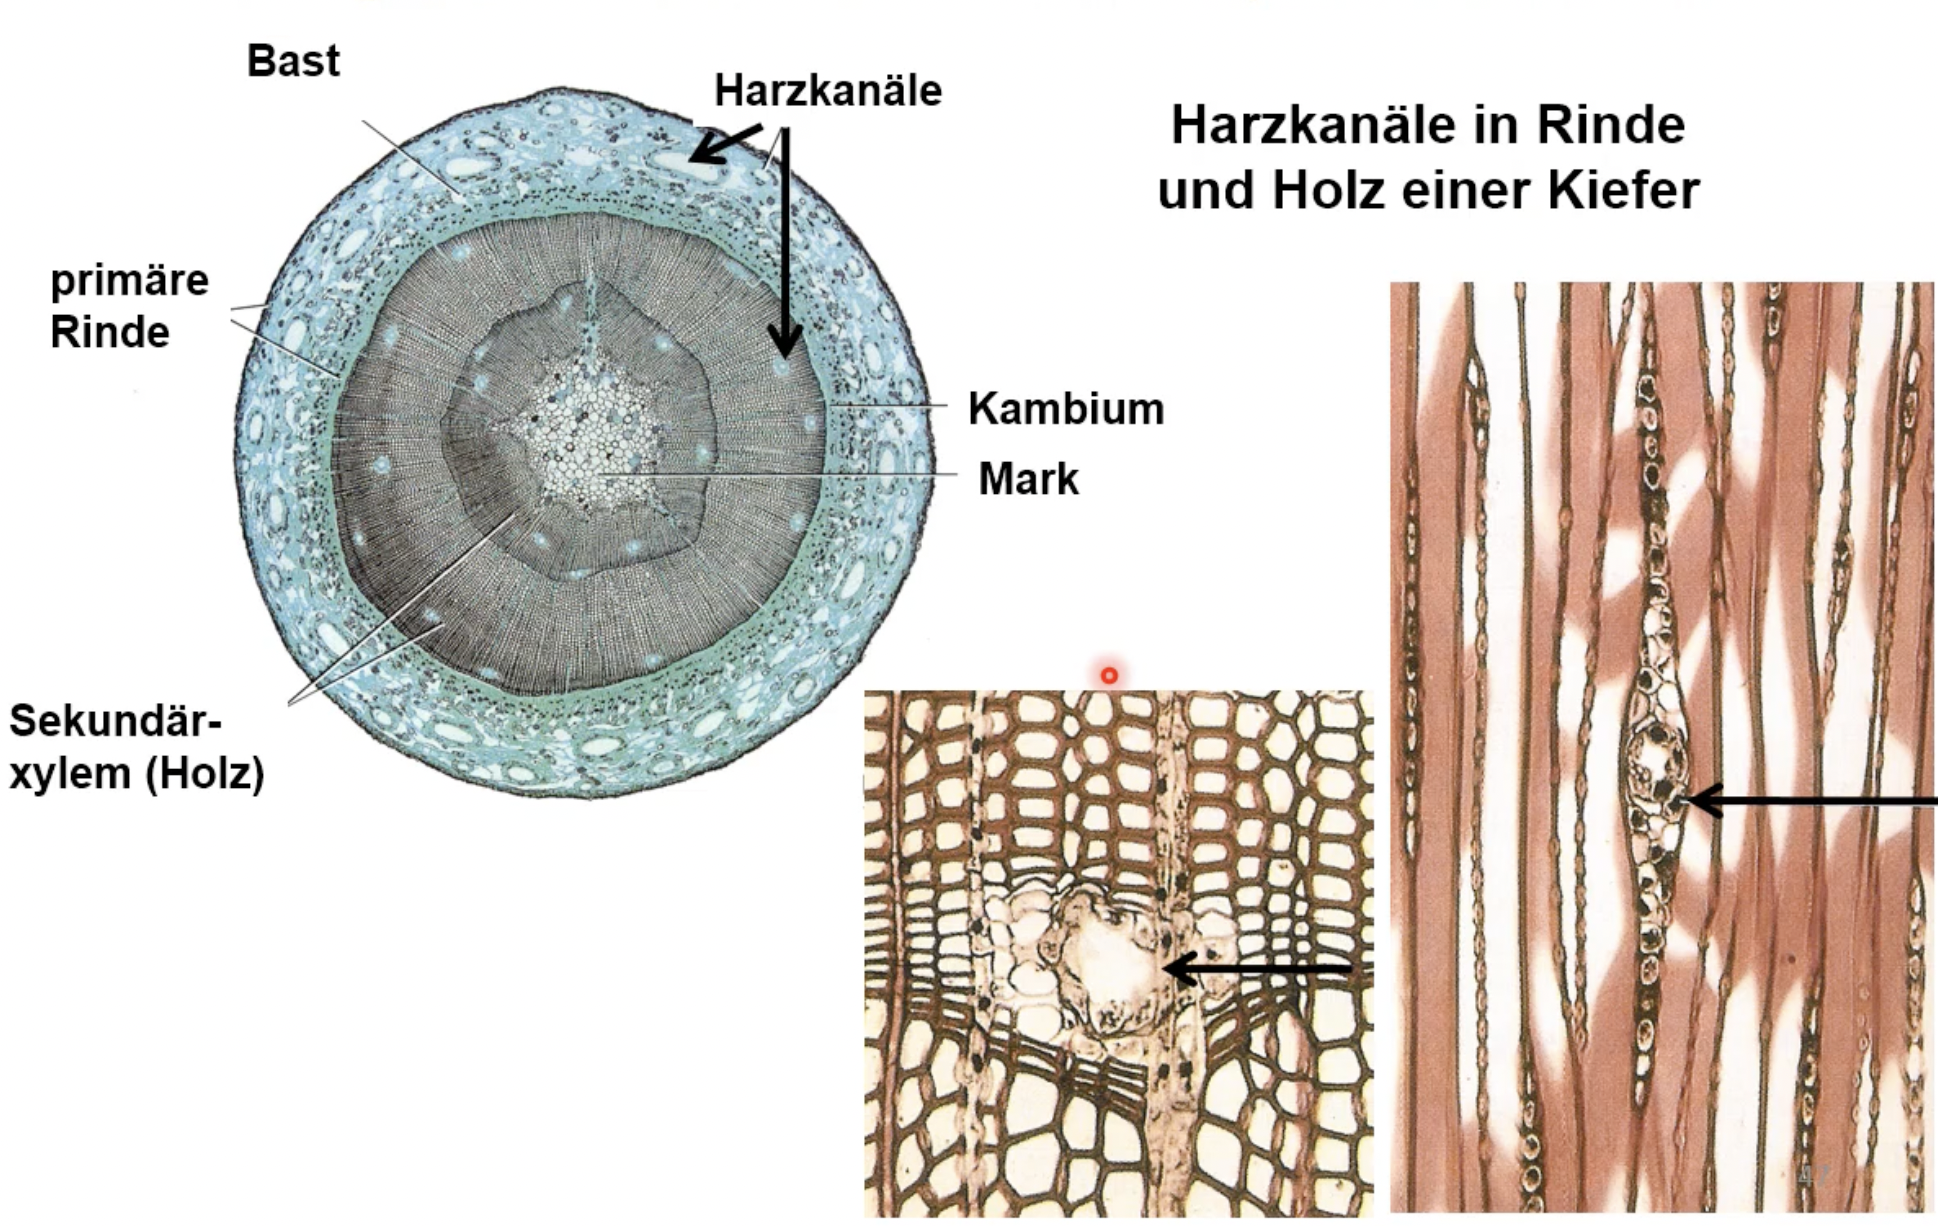
\includegraphics[width=11cm]{lec5/figures/baum.png}
    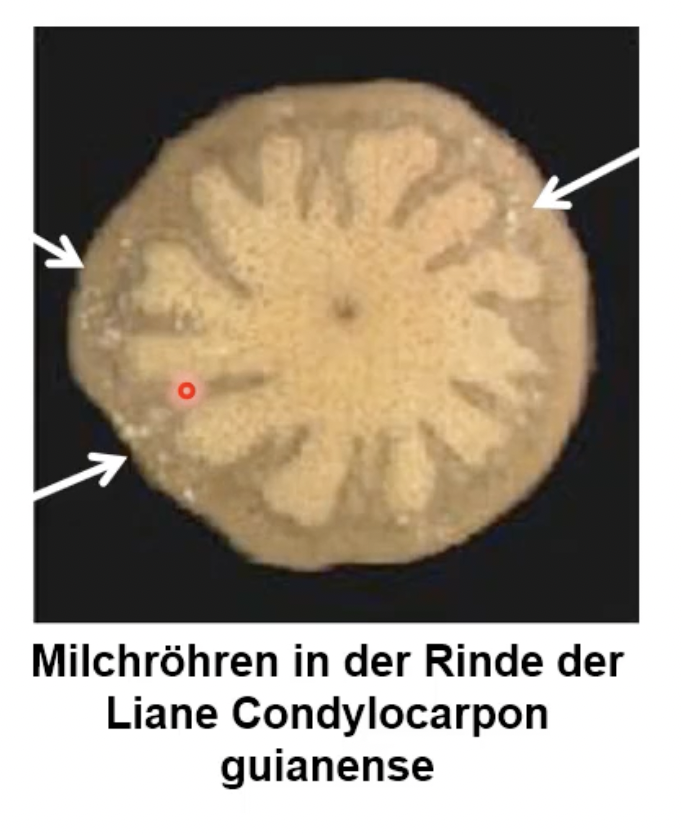
\includegraphics[width=5cm]{lec5/figures/liane.png}
\end{center}
Bei Bäumen wird ausschließlich im \textbf{Kambium} (Stammzellen der Bäume) Material gebildet (linkes Bild). Wenn das Kambium stirbt, stirbt auch der Baum. Nach innen wird Holz produziert, nach außen Bast. Dieser Wachstumsprozess ist deutlich unterschiedlich zu dem der Liane, bei der keine Trennschicht vorhanden ist (rechtes Bild).\\

\vspace*{2\baselineskip}

\textbf{Technische Umsetzung durch Mikrokapseln}\\

Eine Herausforderung der technischen Umsetzung ist es, Mikrokapseln herzustellen, welche mechanisch und thermisch stabil sind, materialgerechte chemische Selbstheilungseigenschaften haben sowie über ein geeignetes Wandmaterial verfügen. Der Stand der bionischen Forschung ist, dass man die Komponenten für die Selbstreparatur produzieren und bereitstellen kann, allerdings die funktionelle Biochemie des Seltsreparaturprozesses sowie die mechanischen Eigenschaften des reparierten Gewebes noch Optimierungsbedarf aufweisen.

\vspace*{2\baselineskip}

\textbf{Erforschung der biochemischen Prozesse der Selbstreparatur von Pflanzen}\\

Der bei Verletzung der Außenschicht austretende Milchsaft des Ficus Benjamina (Gartenfeige) trocknet innerhalb von wenigen Minuten aus und verschließt dadurch die Wunde. Untersuchungen haben Druckverhältnisse von über 8 bar im Inneren der Pflanze ergeben (vergleichbar mit Rennradreifen).\\

\begin{center}
    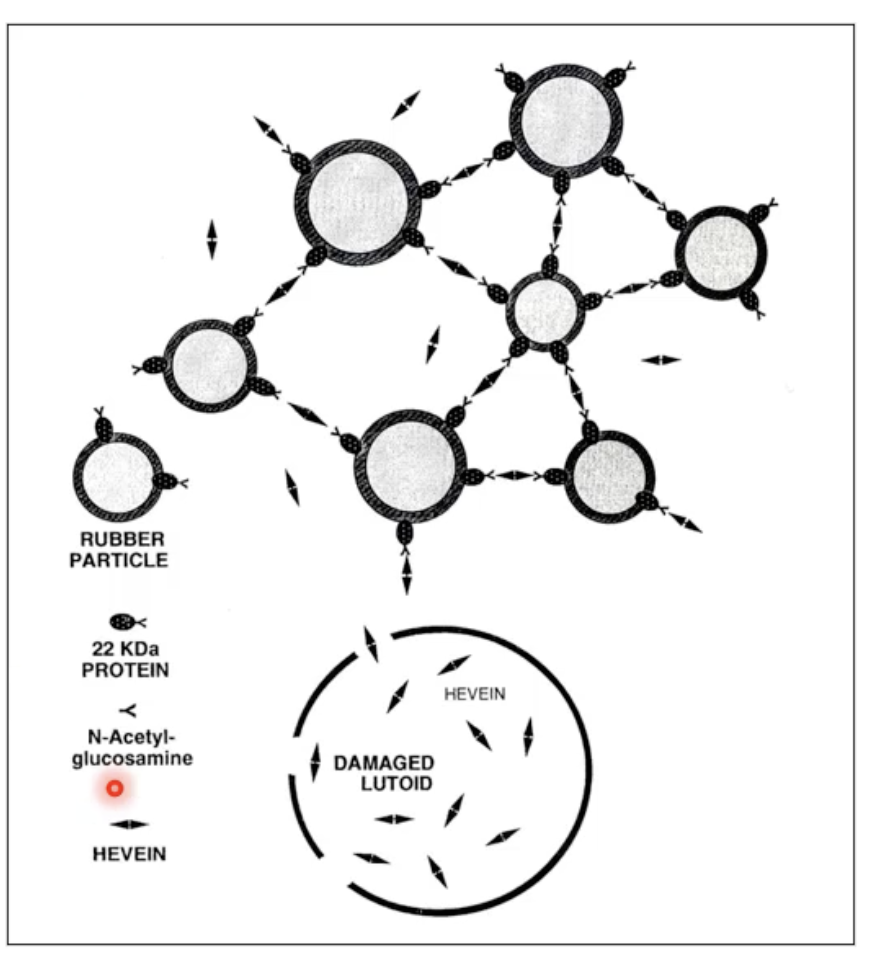
\includegraphics[width=8cm]{lec5/figures/milchsaft.png}
\end{center}
Der \textbf{Milchsaft des Kautschuk-Baumes (Latex)} ist eine Kolloidsuspension von negativ geladenen Latexpartikeln und \textbf{Lutoids} (membranumschlossene Vesikel). Sie befinden sich in Milchröhren (8 bar), im äußeren Bereich des Stammquerschnitts. Die \textbf{Koagulation} des Milchsafts tritt auf, da es durch den \textbf{Druckabfall}, welcher infolge eines Risses in der Außenhülle hervorgerufen wird, zu einem Aufplatzen der Lutoide kommt. Die darin enthaltenen \textbf{Hevein-Proteine} lagern sich an Bindestellen von im Milchsaft vorhandenen Gummipartikeln an und bilden so eine quervernetzte Kettenstruktur \dangersign.\\

\begin{center}
    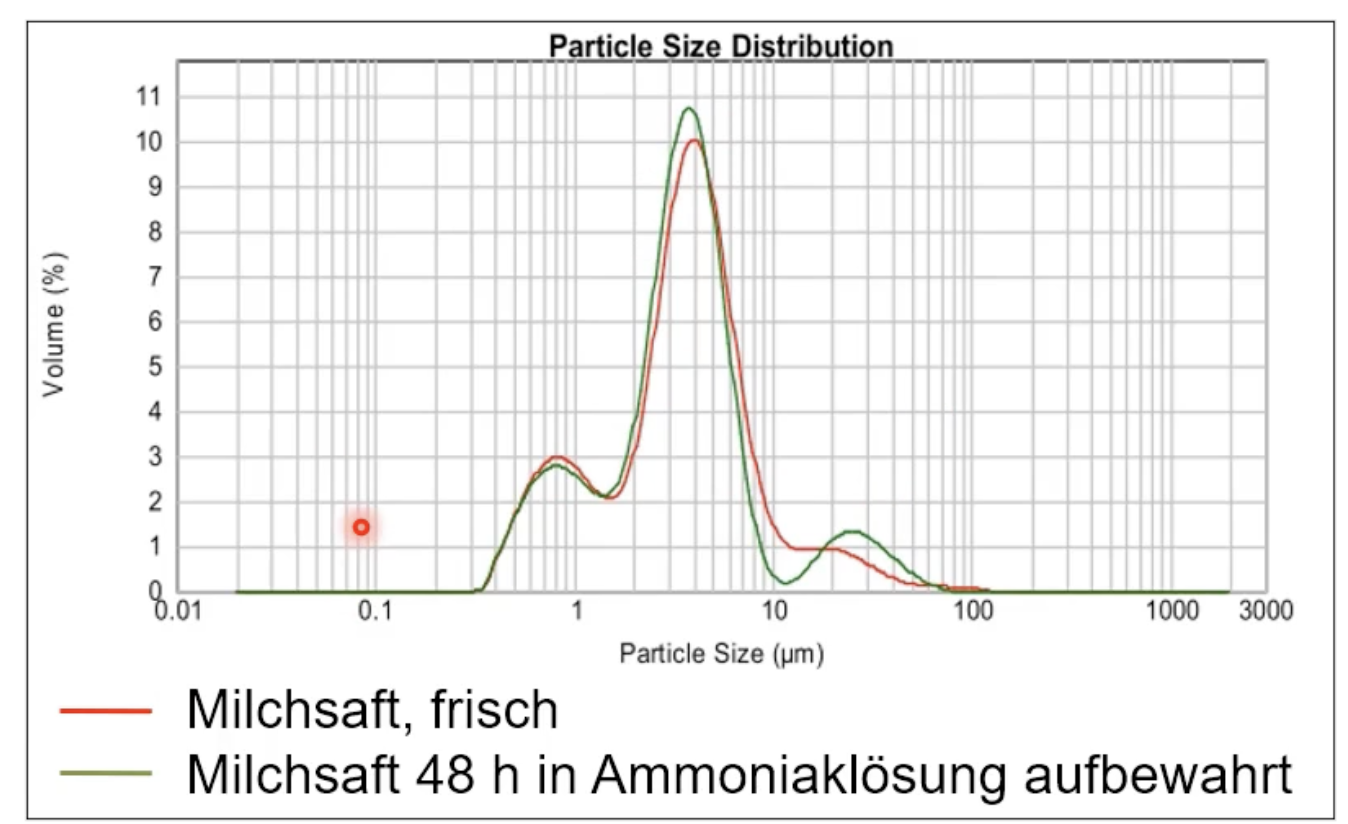
\includegraphics[width=7cm]{lec5/figures/partikel-frisch.png}
    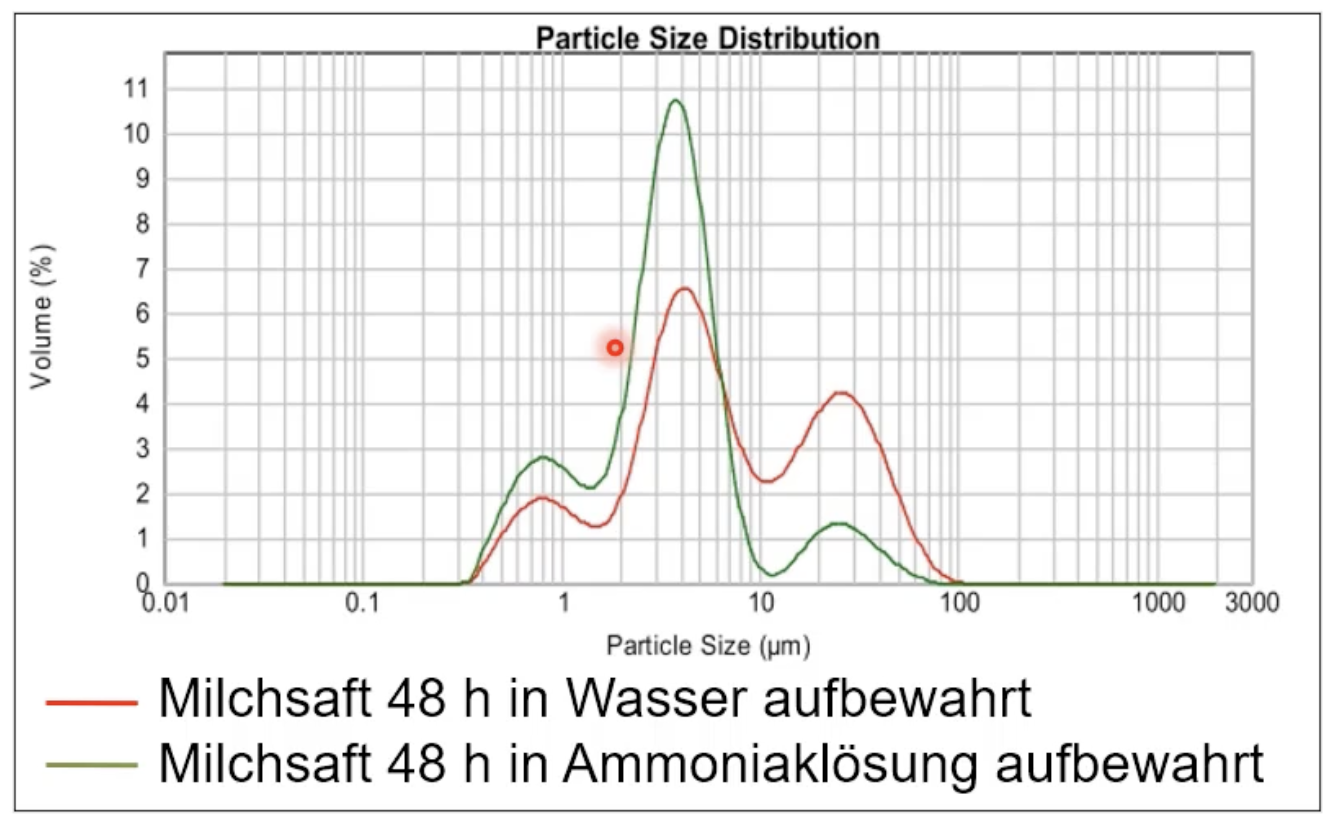
\includegraphics[width=7cm]{lec5/figures/partikel-wasser.png}
\end{center}
Die Koagulation ist pH-abhängig, das Optimum liegt bei einem pH-Wert von 5.5. Dadurch lässt sich mithilfe von Ammoniak die Aushärtung von eingelagertem Natur-Latex (Kautschuk) verhindern. Dieser Effekt ist in den oberen Grafiken für den Milchsaft des Ficus Benjamina zu erkennen und kann auch mithilfe von Tg-IR-Spektrokopie nachgewiesen werden.

\vspace*{2\baselineskip}

\textbf{Erforschung der mechanischen Eigenschaften der Reparaturmaterialien und reparierten Gewebe}\\

Die Tests zur Bestimmung der mechanischen Eigenschaften umfassen:

\begin{itemize}
    \item Zugfestigkeit, E-Modul, vollständige Spannungs-Dehnungsdiagramme mittels Mikro-Zugbühne
    \item Indentationstests auf Mikro- und Nanoebene mittels Mikro-Drucktester und Raster-Kraft-Mikroskop 
\end{itemize}

\begin{center}
    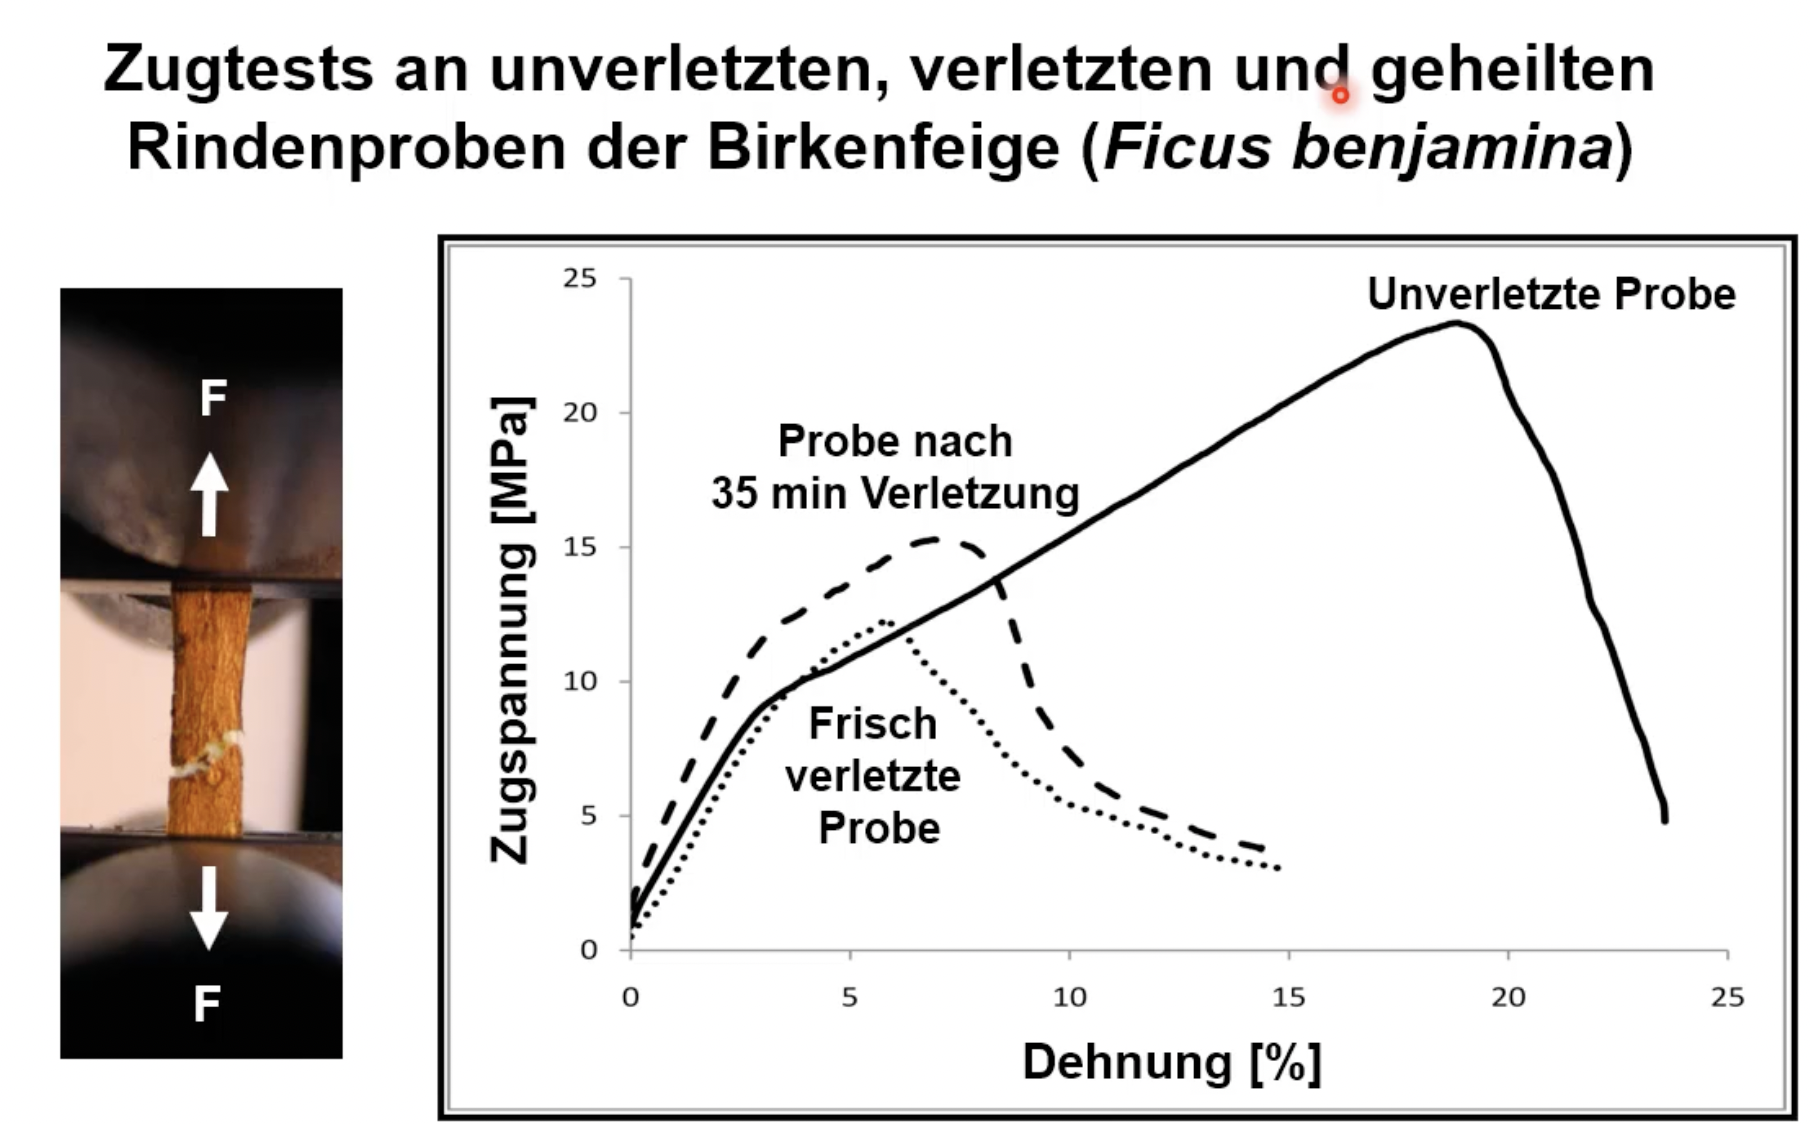
\includegraphics[width=10cm]{lec5/figures/sd.png}
\end{center}
Eine frisch verletzte Probe hat einen deutlich kürzeren Bereich der plastischen Dehnung und damit ein Totalversagen, welches schon bei ca. 25\% der maximalen Dehnung im Vergleich zur unverletzten Probe auftritt. Die Probe mit ausgeheiltem Riss verhält sich ähnlich, kann allerdings in diesem unteren Dehnungsbereich mehr Zugspannung als die unverletzte Probe aushalten. Die \textbf{Reparaturzeit} umfasst dabei bei den meisten Pflanzen ein Minimum von \textbf{10 min}. Da dies für viele technische Anwendungen zu lange ist, wurde ein spezielles Augenmerk auf die \textbf{Glockenblume} gelegt, welche bereits nach \textbf{2 s} signifikante Reparatureffekte aufweist \dangersign.

\vspace*{2\baselineskip}

\subsubsection{Abdichtung nach Vorbild des mechanischen Wundverschlusses bei Pflanzen}

Zugrundeliegendes Problem aus den Ingenieurswissenschaften sind pneumatische Strukturen, welche gegen Luftverlust abgedichtet werden müssen.

\begin{center}
    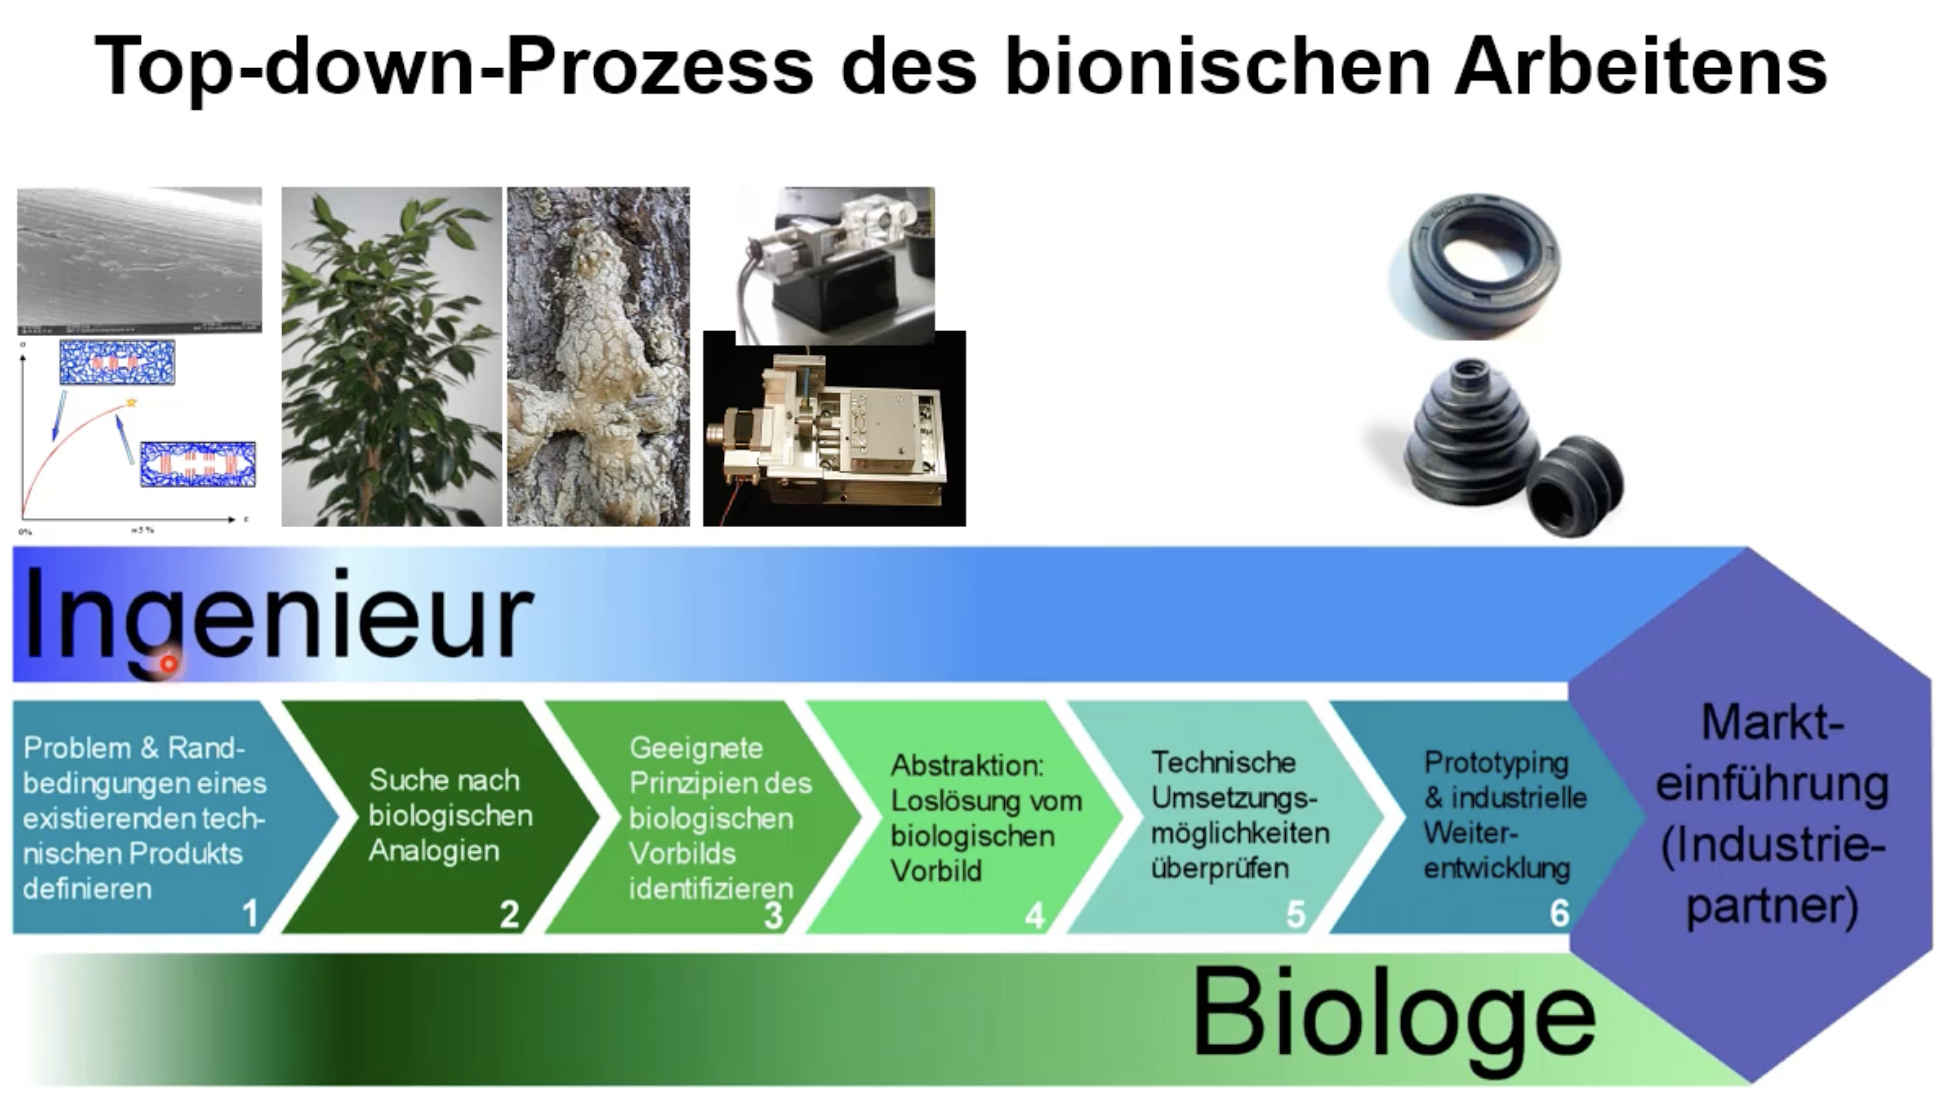
\includegraphics[width=14cm]{lec5/figures/top-down.png}
\end{center}
Motivation für die Erforschung der biochemischen Selbstreparturmechanismen bei Pflanzen ist die Vermeidung eines Luftverlustes bei Beschädigung der Außenhülle von pneumatischen Systemen. Ein relevanter Anwendungsfall hierfür ist die mobile pneumatische Brücke Tensairity (8m Spannweite, 3.5t max.\ Traglast).\\

Als \textbf{biologische Vorbilder wurden schnellwachsende Pflanzen wie bspw.\ die Liane oder der Bohnenstängel} betrachtet. Beim Rissverschluss wird kein neues Material aufgebaut, sondern das bestehende Material verteilt (Änderung der Zellform, Abnahme der Zellwanddicke, gleichbleibendes Zellwandvolumen). Verholzung erfolgt, allerdings auch erst nach mehreren Tagen. Durch Vierpunktbiegung wurde nachgewiesen, dass bei einer Verletzung quer zur Hauptrichtung des Bohnenstängels es erst zu einer signifikanten Abnahme des Biegeelastizitätsmoduls kommt (-40\% nach Tag 3), bis nach 15 Tagen die mechanischen Eigenschaften vollständig wiederhergestellt sind.\\

Abstraktion daraus ist ein technisches Modell mit \textbf{innerer Schaumschicht} aus unter Druck stehenden Zellen (bionische Umsetzung der Selbstreparatur bei Pflanzen) und einer \textbf{äußeren faserverstärkten Membran} der pneumatischen Struktur, wie in der folgenden Abbildung gezeigt. Verschiedene Schaumstrukturen in Zerstörungsprüfungen wurden untersucht. Beschichtung der Membran führt zu einem Reparaturfaktor von 12 (Dauer für Druckabfall 12-mal länger als bei unbeschichteter Membran). Ein \textbf{Überdruck während der Polymerisation} von 2 bar verbessert den Reparaturfaktor auf bis zu 1600.
\\\\
(\dangersign \textit{Worauf basiert die Selbstreparatur bei der Tensairity Luftkissenbrücke? Wie wird ein hoher Reparaturfaktor erreicht?})
\\\\
(\dangersign \textit{Nenne Beispiele für biologische Selbstreparatur + die technische Anwendung})


\begin{center}
    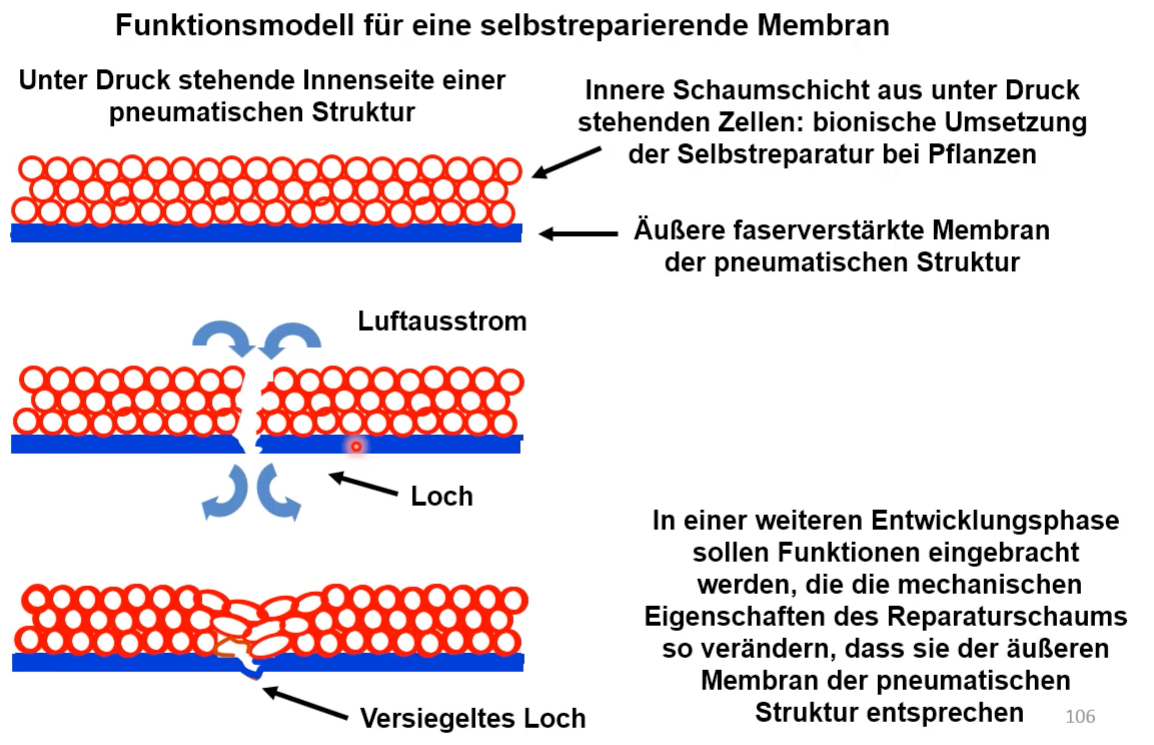
\includegraphics[width=11cm]{lec5/figures/funktionsmodell.png}
\end{center}

\subsubsection{Selbstschärfende Messer nach Vorbild von Nagetierzähnen}

\begin{center}
    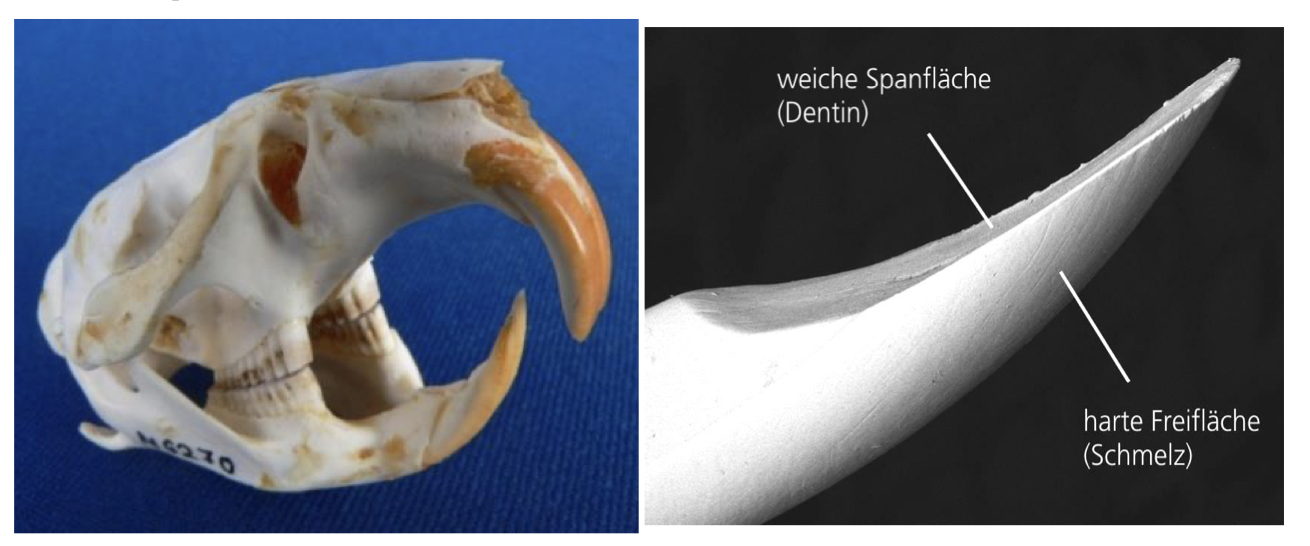
\includegraphics[width=9cm]{lec5/figures/zahn.png}
    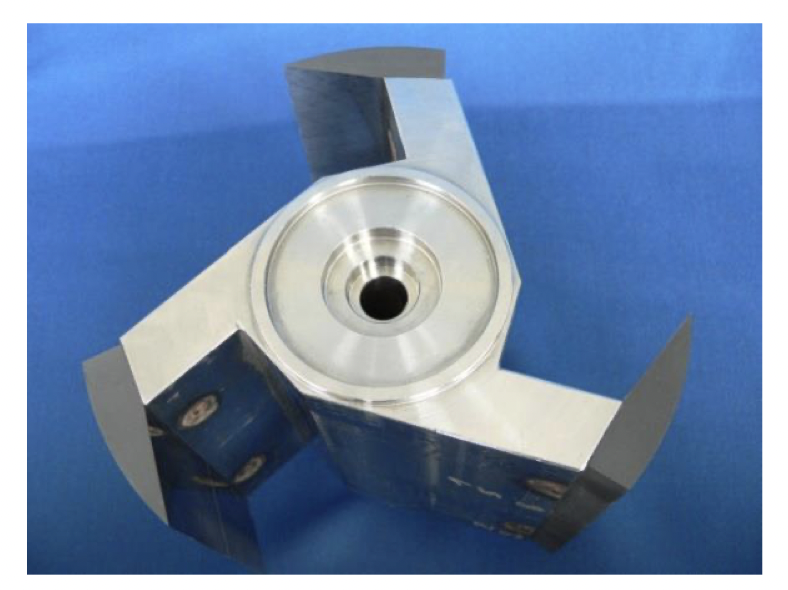
\includegraphics[width=5cm]{lec5/figures/messer.png}
\end{center}
Nagetierzähne wachsen 2-3 mm pro Woche, bleiben allerdings durch einen unterschiedlich starken Abrieb von weicher Spanfläche (Dentin) und harter Freifläche (Schmelz) sowohl in der Länge konstant als auch gleichermaßen an der Zahnspitze scharf. \\

Messer, welche beim Schneiden durch harte Partikel im zu schneidenen Material abstumpfen, müssen zeitaufwändig geschnitten werden. Nach Vorbild des Nagetierzahns wurden daraus selbstschärfende Messer für Industrieschneidemaschinen entwickelt. Ein Nachteil ist, dass immer harte Materialien geschnitten werden müssen um den Effekt der Selbstschärfung auferechtzuerhalten.